\documentclass{article}
\usepackage[utf8]{inputenc}
\usepackage{tikz}

\usetikzlibrary{backgrounds,fit}
\usetikzlibrary{shapes.geometric, arrows, positioning}

\begin{document}


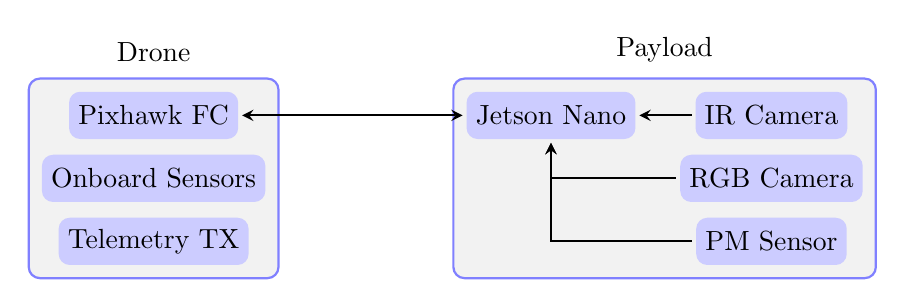
\begin{tikzpicture}[outer sep=0.05cm,node distance=0.8cm,]
\tikzstyle{bigbox} = [draw=blue!50, thick, fill=gray!10, rounded corners, rectangle]
\tikzstyle{box} = [minimum size=0.6cm, rounded corners,rectangle, fill=blue!20]
\tikzstyle{arrow} = [thick,->,>=stealth]

% Drone
\node[box] (pixhawk) {Pixhawk FC};
\node[box, below of=pixhawk] (sensors) {Onboard Sensors};
\node[box, below of=sensors] (tx) {Telemetry TX};
%
\begin{pgfonlayer}{background}
  \node[bigbox, label={Drone}] [fit = (pixhawk) (sensors) (tx)] (dron) {};
\end{pgfonlayer}

% Payload
% \node[box,below=of sensors.west, anchor=west, yshift=-1cm] (jetson) {Jetson Nano};
\node[box,right=of pixhawk.east, anchor=west, xshift=2cm] (jetson) {Jetson Nano};
\node[box,right of=jetson, xshift=2cm] (ir_cam) {IR Camera};
\node[box,below of=ir_cam] (rgb_cam) {RGB Camera};
\node[box,below of=rgb_cam] (pms) {PM Sensor};
%
\begin{pgfonlayer}{background}
  \node[bigbox, label={Payload}] [fit = (jetson) (rgb_cam) (pms)] (payload) {};
  
\end{pgfonlayer}

% \draw [arrow] (payload) -- (dron);
\draw [arrow] [thick,<->,>=stealth] (jetson) -- (pixhawk);

\draw [arrow] [thick,<-,>=stealth] (jetson) |- (pms);
\draw [arrow] [thick,<-,>=stealth] (jetson.south) |- (rgb_cam);
\draw [arrow] [thick,<-,>=stealth] (jetson) -- (ir_cam);

%
\end{tikzpicture}

\end{document}